% Template cho một chương

\chapter{Adversarial regularization for image classification} % Tên của chương

\label{Chapter2} % Thay X bằng số chương tương ứng; để trích dẫn chương này ở chỗ nào đó trong bài, hãy sử dụng lệnh \ref{ChapterX} 

%----------------------------------------------------------------------------------------
%	MỤC 1
%----------------------------------------------------------------------------------------

\section{Đặt vấn đề}

Ở chương một chúng ta đã đi qua tổng quan về TensorFLow và Neural Structured Learning. Tuy nhiên để làm rõ hơn về hiệu quả của Neural
Structured Learning, chúng ta cần thực nghiệm trên một bài toán thực tế. Vì vậy ta sẽ ứng dụng Neural Structured Learning và chính xác hơn là Adversarial 
Regularization for Image Classification.

Dựa trên tập dữ liệu có sẵn của thư viện TensorFlow MNIST, chúng ta sẽ thực hiện một bài toán phân loại ảnh chữ số viết tay. Tập dữ liệu bao gồm 70.000 ảnh
chữ số viết tay được chia thành 60.000 ảnh để huấn luyện và 10.000 ảnh để kiểm tra. Mỗi ảnh có kích thước 28x28 pixel và được biểu diễn dưới dạng một mảng
2 chiều 28x28. Mỗi phần tử trong mảng này là một giá trị từ 0 đến 255 biểu diễn độ sáng của một pixel. Để thuận tiện cho việc huấn luyện, chúng ta sẽ chuyển đổi
mỗi ảnh thành một mảng 1 chiều 784 phần tử. Để đơn giản hơn, chúng ta sẽ chia tập dữ liệu thành 2 tập huấn luyện và kiểm tra. Tập huấn luyện sẽ bao gồm 60.000 ảnh 
và tập kiểm tra sẽ bao gồm 10.000 ảnh. Mỗi ảnh sẽ được gán nhãn là một số từ 0 đến 9 tương ứng với chữ số viết tay. 

\begin{figure}[h!]
    \centering
    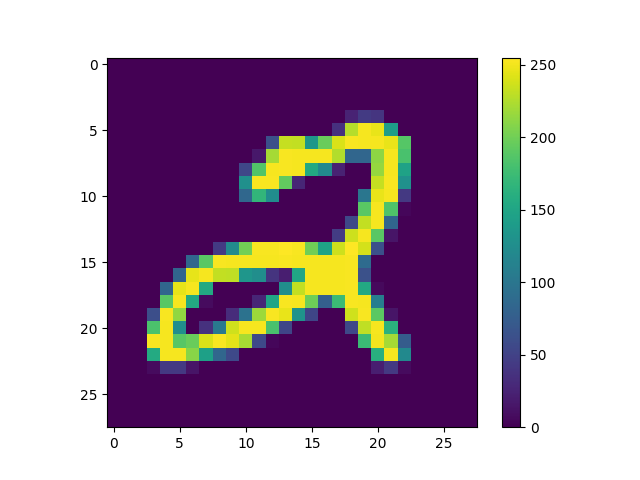
\includegraphics[width=0.6\linewidth]{Image/data.png}
    \caption{Ảnh chữ số viết tay được lấy từ tập dữ liệu MNIST}
    \label{Hình 2.1: GẢnh chữ số viết tay được lấy từ tập dữ liệu MNIST}
\end{figure}


Chúng ta sẽ thực hiện xây dựng và đào tạo một mạng neural đơn giản và một mạng neural sử dụng Adversarial Regularization. Sau đó chúng ta sẽ so sánh kết quả 
dự đoán của 2 mạng neural này để thấy được hiệu quả của Neural Structured Learning. Sau khi đào tạo và dự đoán thử trên tập dữ liệu có sẵn của TensorFlow, thì
ta sẽ thử viết tay một vài chữ số và để cho mạng neural dự đoán xem nó có thể dự đoán chính xác không.

Với những thư viện đồ sộ và khả năng làm việc với các ma trận tốt, Python là ngôn ngữ được lựa chọn để thực hiện ý tưởng trên. Cùng với đó là các thư viện như numpy, matplotlib và
đặc biệt là TensorFlow với API keras và Neural structed learning.





%----------------------------------------------------------------------------------------
%	MỤC 2
%----------------------------------------------------------------------------------------

\section{Thực nghiệm}

\subsection{Cài đặt môi trường}

Bước đầu tiên cần cài đặt biến môi trường và các thư viện cần thiết. Cài đặt phiên bản python3 và editor hoặc IDE để viết mã như Pycharm hoặc VScode.
Sau đó, trên command line chạy dòng lệnh 'pip install -r Setup.txt' để tiến hành cài đặt các thư viện cần thiết. File "Setup.txt" là file chứa các thư viện 
cần cài đặt.

\subsection{Viết mã}
\textbf{Import thư viện}
% insert code python
\begin{lstlisting}[language=Python]
    import tensorflow as tf
    import numpy as np
    import neural_structured_learning as nsl
    import matplotlib.pyplot as plt
    import tensorflow_datasets as tfds
\end{lstlisting}

\textbf{Khai báo các tham số}
% insert code python
\begin{lstlisting}[language=Python]
    input_shape = [28, 28, 1]
    num_classes = 10
    conv_filters = [32, 64, 64]
    kernel_size = (3, 3)
    pool_size = (2, 2)
    num_fc_units = [64]
    batch_size = 32
    epochs = 5
    adv_multiplier = 0.2
    adv_step_size = 0.2
    adv_grad_norm = 'infinity'
\end{lstlisting}

Khai báo các tham số cần thiết cho việc xây dựng mạng neural và đào tạo. Các tham số được khai báo như sau:

Đầu vào và đầu ra:
\begin{itemize}
    %highlight Item name
    \item \textbf{input\_shape}: Hình dạng của tensor đầu vào. Mỗi hình ảnh có kích thước 28x28pixel và có 1 kênh màu.
    \item \textbf{num\_classes}: Số lượng lớp đầu ra. Trong bài toán này là 10 lớp từ 0 đến 9.
\end{itemize}

Các tham số để xây dựng mô hình mạng neural:
\begin{itemize}
    %highlight Item name
    \item \textbf{conv\_filters}: Số lượng lọc cho mỗi lớp tích chập. Mỗi lớp tích chập có số bộ lọc bao gồm 32,64,64.
    \item \textbf{kernel\_size}: Kích thước của kernel tích chập 2D. Mỗi kernel có kích thước 3x3.
    \item \textbf{pool\_size}: Các yếu tố để thu nhỏ hình ảnh trong mỗi lớp tổng tối đa. Mỗi pooling có kích thước 2x2.
    \item \textbf{num\_fc\_units}: Số lượng đơn vị ẩn của mỗi lớp fully connected. Mỗi lớp fully connected có 64 đơn vị ẩn. Nghĩa là chiều rộng của mỗi lớp được kết nối đầy đủ.
\end{itemize}

Các tham số để đào tạo mô hình:
\begin{itemize}
    \item \textbf{batch\_size}: Kích thước batch. Mỗi batch có 32 hình ảnh. Là số lượng bức ảnh được đưa vào mạng neural mỗi lần.
    \item \textbf{epochs}: Số lần huấn luyện. Mỗi lần sẽ duyệt qua tất cả các hình ảnh trong tập dữ liệu.
    \item \textbf{adv\_multiplier}: Trọng số tổn thất do nhiễu loạn đối nghịch gây ra trong mục tiêu huấn luyện, so với tổn thất của mô hình gốc(tổn thất được gắn nhãn).
    \item \textbf{adv\_step\_size}: Độ lớn của nhiễu loạn đối nghịch.
    \item \textbf{adv\_grad\_norm}: Định mức để đo mức độ nhiễu loạn của đối nghịch. %Có 3 giá trị là 'infinity', 'l2', 'l1'.
\end{itemize}

\textbf{Tải dữ liệu MNIST}
% insert code python
\begin{lstlisting}[language=Python]
    data_train, data_test = tfds.load('mnist', split=['train', 'test'])
\end{lstlisting}

Bộ dữ liệu MNIST chứa hình ảnh thang độ xám của các chữ số viết tay từ 0 dến 9. Mỗi hình ảnh hình ảnh hiển thị một chữ số ở độ phân giải thấp 28x28 pixel.
Nhiệm vụ liên quan là phân loại hình ảnh thành 10 loại, mỗi loại tương ứng với một chữ số từ 0 đến 9.

Bộ dữ liệu đã có sẵn trong thư viện TensorFlow Datasets (TFDS) và có thể được tải xuống và xây dựng tệp tf.data.Dataset.
Tập dữ liệu đã tải bao gồm hai tập con :
\begin{itemize}
    \item \textbf{train}: Tập dữ liệu huấn luyện với 60000 ảnh.
    \item \textbf{test}: Tập dữ liệu kiểm tra với 10000 ảnh.
\end{itemize}

Các dữ liệu trong cả hai tập đều được lưu trữ dưới dạng dictionary với hai khóa:
\begin{itemize}
    \item \textbf{image}: Là các mảng pixel 28x28 chứa các giá trị từ 0 đến 255.
    \item \textbf{label}: Nhãn thật của hình ảnh, là một số nguyên từ 0 đến 9.
\end{itemize}

\begin{lstlisting}[language=Python]
    def normalize(features):
        features['image'] = tf.cast(features['image'], dtype=tf.float32) / 255.0
        return features

    def convert_to_tuples(features):
        return features['image'], features['label']

    def convert_to_dictionaries(image, label):
        return {'image': image, 'label': label}

    data_train = data_train.map(normalize).shuffle(10000).batch(batch_size).map(convert_to_tuples)
    data_test = data_test.map(normalize).batch(batch_size).map(convert_to_tuples)

\end{lstlisting}

Để làm cho mô hình ổn định về số lượng, chúng ta chuẩn hóa các giá trị pixel từ [0,255] thành [0, 1] bằng cách ánh xạ tập dữ liệu qua hàm normalize(). Sau khi xáo 
trộn tập huấn luyện và chia theo nhóm, chúng ta chuyển đổi các ví dụ thành các bộ dữ liệu đặc trưng (image, label) để huấn luyện mô hình cơ sở. Chúng ta 
cũng cung cấp một hàm chức năng để chuyển đổi từ bộ sang từ điển để sử dụng sau này.

\textbf{Xây dựng và đào tạo mô hình cơ bản}

Mô hình cơ bản sẽ là một mạng thần kinh bao gồm 3 lớp tích chập, theo sau là 2 lớp được kết nối đầy đủ ( với các tham số như được định nghĩa trong phần khai báo tham số). 
Trong đó các lớp tích chập sẽ có hàm kích hoạt activation là 'relu' còn hai lớp theo sau thì một lớp có hàm kích hoạt là 'relu'và lớp output sẽ là 'softmax'. Lớp output sử dụng 
activation 'softmax' để đánh giá xác suất phân loại dữ liệu đầu vào và tính toán trọng số cho dữ liệu.
Chúng ta tạo hàm build\_model() để thuận tiện cho việc tái sử dụng khi khởi tạo mô hình khác. 
Ở đây chúng ta xác định nó bằng các hàm API của Keras. 

\begin{lstlisting}[language=Python]
    def build_model():
        inputs = tf.keras.Input(shape=input_shape, dtype=tf.float32, name='image')
        x = inputs
        for i, num_filters in enumerate(conv_filters):
            x = tf.keras.layers.Conv2D(num_filters, kernel_size, activation='relu')(x)
            if i < len(conv_filters) - 1:
                x = tf.keras.layers.MaxPooling2D(pool_size)(x)
        x = tf.keras.layers.Flatten()(x)
        for num_units in num_fc_units:
            x = tf.keras.layers.Dense(num_units, activation='relu')(x)
        outputs = tf.keras.layers.Dense(num_classes, activation='softmax')(x)
        return tf.keras.Model(inputs=inputs, outputs=outputs)

    model_base = build_model()
\end{lstlisting}

Sau khi xây dựng model thì chúng ta sẽ tiến hành đào tạo và đánh giá model. Với hàm tối ưu hóa 'Adam' như đã giới thiệu ở phần trước, hàm mất mát 'SparseCategoricalCrossentropy'
và đánh giá 'SparseCategoricalAccuracy'. Sau khi đào tạo xong chúng ta sẽ đánh giá model bằng hàm evaluate() và in ra độ chính xác của model.

\begin{lstlisting}[language=Python]
model_base.compile(
    optimizer=tf.keras.optimizers.Adam(),
    loss=tf.keras.losses.SparseCategoricalCrossentropy(),
    metrics=[tf.keras.metrics.SparseCategoricalAccuracy()])
model_base.summary()

model_base_history = model_base.fit(data_train, epochs=epochs)

results = model_base.evaluate(data_test)
named_results = dict(zip(model_base.metrics_names, results))
print('\naccuracy:', named_results['sparse_categorical_accuracy'])

\end{lstlisting}

\begin{figure}[ht]
\centering
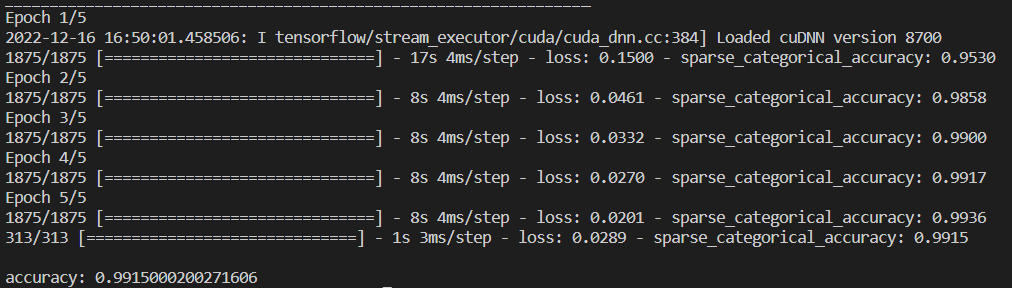
\includegraphics[width=\textwidth]{Image/base_acc.png}
\caption{Accuracy}
\label{fig2.2:Độ chính xác của mô hình cơ bản}
\end{figure}

Chúng ta có thể thấy rằng mô hình cơ bản đạt được độ chính xác lên đến 99,15\% trên bộ thử nghiệm. Từ đó cho thấy dữ liệu đào tạo và 
mô hình đào tạo là khá tốt. Tuy nhiên cần phải sử dụng các tập dữ liệu khác để đánh giá mô hình một cách chính xác hơn.

\textbf{Xây dựng và đào tạo mô hình Adversarial-regularized }

Chúng ta sẽ xây dựng mô hình mạng neural đối nghịch bằng cách kết hợp adversarial training vào mô hình keras và sử dụng khung Neural Structured Learning (NSL).
Mô hình cơ sở được bao bọc để tạo một mô hình mới \textbf{tf.Keras.Model}, có mục tiêu đào tạo bao gồm adversarial regularization.

Đầu tiên, chúng tôi tạo một đối tượng cấu hình với tất cả cáctham số có liên quan bằng cách sử dụng hàm chức năng \textbf{nsl.configs.make\_adv\_reg\_config} có sẵn trong thư viện NSL.

\begin{lstlisting}[language=Python]
    adv_config = nsl.configs.make_adv_reg_config(multiplier=adv_multiplier, 
        adv_step_size=adv_step_size, 
        adv_grad_norm=adv_grad_norm)
\end{lstlisting}

Ở đây chúng ta sẽ tạo một mô hình cơ bản mới \textbf{base\_adv\_model} để mô hình hiện tại (\textbf{model\_base}) dùng để so sánh sau này.

Bây giờ chúng ta có thể bọc một mô hình cơ sở bằng \textbf{AdversarialRegularization} bằng cách sử dụng hàm chức năng
có sẵn \textbf{nsl.keras.AdversarialRegularization}.

\begin{lstlisting}[language=Python]
    base_adv_model = build_model()
    model_adv = nsl.keras.AdversarialRegularization(
        base_adv_model,
        label_keys=['label'],
        adv_config=adv_config)

    data_train_adv = data_train.map(convert_to_dictionaries)
    data_test_adv = data_test.map(convert_to_dictionaries)
\end{lstlisting}

Trả về \textbf{adv\_model} là một đối tượng có kiểu \textbf{tf.keras.Model}, có mục tiêu đào tạo bao gồm phần regularization và mất mát của adveresarial. Để tính toán tổn thất đó, mô hình phải có quyền truy cập 
vào thông tin nhãn (feature label), ngoài đầu vào thông thường (feature image). Vì lý do này, chúng ta sẽ chuyển đổi các mẫu trong tập dữ liệu trở lại kiểu dictionary. Và chúng ta cho mô 
hình biết tính năng nào chứa thông tin nhãn thông qua tham số \textbf{label\_keys}.

Tiếp theo, chúng ta sẽ biên dịch, đào tạo và đánh giá mô hình chính quy hóa đối thủ. Với các hàm tối ưu, mất mát, và đánh giá độ chính xác tương tự như khi đào tạo mô hình cơ bản.
Có thể có các cảnh báo như "Output missing from loss dictionary", điều này không sao cả vì \textbf{adv\_model} không dựa vào triển khai cơ sở để tính tổng tổn thất.



\begin{lstlisting}[language=Python]
    model_adv.compile(
        optimizer=tf.keras.optimizers.Adam(),
        loss=tf.keras.losses.SparseCategoricalCrossentropy(),
        metrics=[tf.keras.metrics.SparseCategoricalAccuracy()])

    model_adv_history = model_adv.fit(data_train_adv, epochs=epochs)
    
    adv_results = model_adv.evaluate(data_test_adv)
    named_adv_results = dict(zip(model_adv.metrics_names, adv_results))
    print('\naccuracy:', named_adv_results['sparse_categorical_accuracy'])

\end{lstlisting}

\begin{figure}[h!]
    \centering
    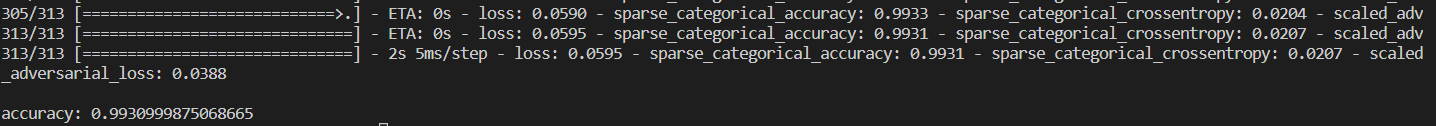
\includegraphics[width=\textwidth]{Image/adv_acc.png}
    \caption{Độ chính xác của mô hình Adversarial-regularized.}
    \label{fig 2.3:Độ chính xác của mô hình Adversarial-regularized}
\end{figure}

Chúng ta có thể thấy rằng mô hình Adversarial-regularized cũng hoạt động rất tốt (độ chính xác 99,31\%) trên tập thử nghiệm. Tuy độ chính xác có nhỉnh hơn một xíu so với mô hình cơ bản
nhưng không quá nhiều.

Chúng ta sẽ đưa ra đồ thị sự thay đổi của độ chính xác qua mỗi lần học tập trên tập dữ liệu thử nghiệm của cả hai mô hình để dễ dàng quan sát hơn.
\begin{lstlisting}[language=Python]
    plt.plot(model_base_history.history['sparse_categorical_accuracy'])
    plt.plot(model_adv_history.history['sparse_categorical_accuracy'])
    plt.title('model accuracy')
    plt.ylabel('accuracy')
    plt.xlabel('epoch')
    plt.legend(['base', 'adversarial'], loc='upper left')
    plt.show()
\end{lstlisting}

\begin{figure}[h!]
    \centering
    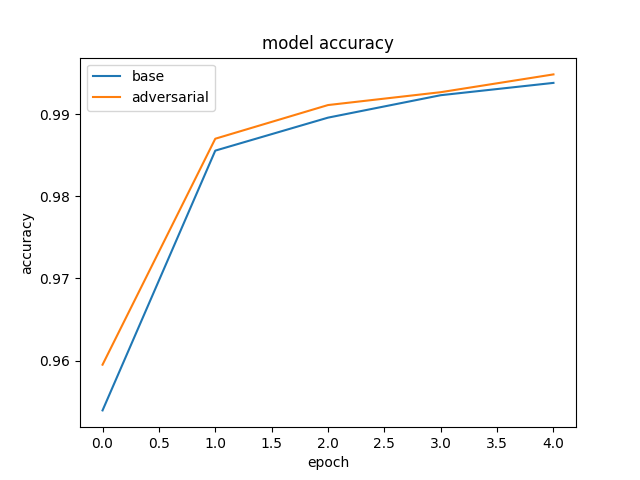
\includegraphics[width=0.7\textwidth]{Image/plt.png}
    \caption{Đồ thị độ chính xác của hai mô hình qua từng lần học.}
    \label{fig 2.4:Đồ thị độ chính xác của hai mô hình qua từng lần học.}
    
\end{figure}

Từ đồ thị, ta thấy đường cong độ chính xác của mô hình Adversarial-regularized và mô hình cơ bản có xu hướng tương tự nhau. Mô hình adversarial-regularized có nhỉnh hơn một chút nhưng chênh lệch là không quá nhiều. 
Điều này là do cả hai mô hình đều sử dụng các hàm tối ưu, mất mát và đánh giá tương tự nhau.

\textbf{So sánh độ chính xác của hai mô hình dưới các mẫu nhiễu loạn đối nghịch}

Bây giờ chúng ta so sánh mô hình cơ sở và mô hình Adversarial-regularized về khả năng phán đoán chính xác dưới sự nhiễu loạn của các mẫu đối nghịch.
Chúng ta sẽ sử dụng hàm chức năng \textbf{AdversarialRegularization.perturb\_on\_batch()} để tạo các mẫu nhiễu loạn đối nghịch. Để có thể sánh được độ chính xác của hai mô hình,
ta sẽ phải bọc mô hình cơ bản bằng \textbf{AdversarialRegularization}. Các biến mà mô hình cơ bản đã học trước đó sẽ không bị thay đổi miễn là chúng ta không gọi hàm đào tạo \textbf{fit()}.

\begin{lstlisting}[language = Python]
    ref_model = nsl.keras.AdversarialRegularization(
        model_base,
        label_keys=['label'],
        adv_config=adv_config)


    ref_model.compile(
        optimizer=tf.keras.optimizers.Adam(),
        loss=tf.keras.losses.SparseCategoricalCrossentropy(),
        metrics=[tf.keras.metrics.SparseCategoricalAccuracy()])
\end{lstlisting}

Tiếp theo chúng ta sẽ đánh giá và so sánh khả năng phán đoán của hai mô hình trên các mẫu đối nghịch.
Ở đây chúng ta lấy \textbf{adv\_model.base\_model} để có cùng định dạng đầu vào (không yêu cầu thông tin nhãn) làm mô hình cơ sở. Các biến đã học trong \textbf{adv\_model.base\_model} giống như các biến 
trong \textbf{adv\_model}.

\begin{lstlisting}[language = Python]
    models_to_evaluate = {
        'base': model_base,
        'adversarial': model_adv.base_model,
    }

    metrics = {
        name: tf.keras.metrics.SparseCategoricalAccuracy()
        for name in models_to_evaluate.keys()
    }    
\end{lstlisting}

Tiếp theo chúng ta sẽ tạo các ví dụ nhiễu loạn và đánh giá các mô hình với chúng. Chúng ta lưu các hình ảnh, nhãn và dự đoán bị nhiễu vào 3 mảng perturbed\_imgs,labels,predictions để trực 
quan hóa trong phần sau để có cách nhìn rõ hơn về khả năng phán đoán của hai mô hình. Các mẫu nhiễu loạn được tạo ra từ tập dữ liệu test và
được chuẩn hóa để chúng có cung kích thước với các mẫu thông thường bằng hàm chức năng \textbf{tf.clip\_by\_value}.


\begin{lstlisting}[language = Python]
    perturbed_imgs,labels,predictions = [],[],[]

    for batch in data_test_adv:
        perturbed_batch = ref_model.perturb_on_batch(batch)
        perturbed_batch['image'] = tf.clip_by_value(perturbed_batch['image'], 0, 1)

        y_true = perturbed_batch.pop('label')
        perturbed_imgs.append(perturbed_batch['image'].numpy())
        labels.append(y_true.numpy())
        predictions.append({})

        for name, model in models_to_evaluate.items():
            y_pred = model(perturbed_batch)
            metrics[name].update_state(y_true, y_pred)
            predictions[-1][name] = tf.argmax(y_pred, axis=-1).numpy()

    for name, metric in metrics.items():
        print(f'{name} accuracy: {metric.result().numpy()}')

\end{lstlisting}

\begin{figure}[h!]
    \centering
    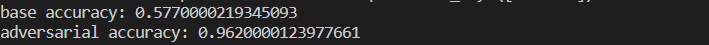
\includegraphics[width=\textwidth]{Image/acc.png}
    \caption{Độ chính xác của hai mô hình trên mẫu nhiễu loạn đối nghịch.}
    \label{fig 2.5:Độ chính xác của hai mô hình trên mẫu nhiễu loạn đối nghịch.}
    
\end{figure}

Từ hình 2.5 Chúng ta có thể thấy rằng độ chính xác của mô hình cơ bản giảm đáng kể (từ 99,15\% xuống còn khoảng 57,7\%) khi đầu vào bị nhiễu. Mặt khác, 
độ chính xác của mô hình Adversarial-regularized chỉ giảm một chút (từ 99,31\% xuống 96,2\%). Điều này chứng tỏ tính hiệu quả của việc học đối thủ trong 
việc cải thiện độ chính của mô hình và khả năng hoạt động tốt của mô hình trên những tập dữ liệu nhiều nhiễu.

\textbf{Trực quan hóa các mẫu nhiễu loạn đối nghịch}

Chúng ta sẽ chọn ra một batch ngẫu nhiên trong mảng perturbed\_imgs đã lưu ở trên để trực quan hóa, ở đây batch được chọn là batch thứ 5.
Sử dụng thư viện \textbf{matplotlib} để hiển thị các hình ảnh và hiển thị các dự đoán của hai mô hình và kiểm tra xem mô hình đoán có đúng không so với
nhãn thật.


\begin{lstlisting}[language = Python]
    batch_index = 5

    batch_images = perturbed_imgs[batch_index]
    batch_labels = labels[batch_index]
    batch_predictions = predictions[batch_index]

    n_columns = 5
    n_rows = (batch_size + n_columns - 1) // n_columns

    print('acc in batch %d: ' % batch_index, end='')
    for name,pred in batch_predictions.items():
        print('%s model: %d / %d' % (name, np.sum(batch_labels == pred), batch_size))

    plt.figure(figsize=(n_columns * 2, n_rows * 2))
    for i,(img,y) in enumerate(zip(batch_images, batch_labels)):
        y_base = batch_predictions['base'][i]
        y_adv = batch_predictions['adversarial'][i]
        plt.subplot(n_rows, n_columns, i + 1)
        plt.title('true: %d, base: %d, adv: %d' % (y, y_base, y_adv))
        plt.imshow(img)
        plt.axis('off')

    plt.tight_layout()
    plt.show()

    
\end{lstlisting}

\begin{figure}[h!]
    \centering
    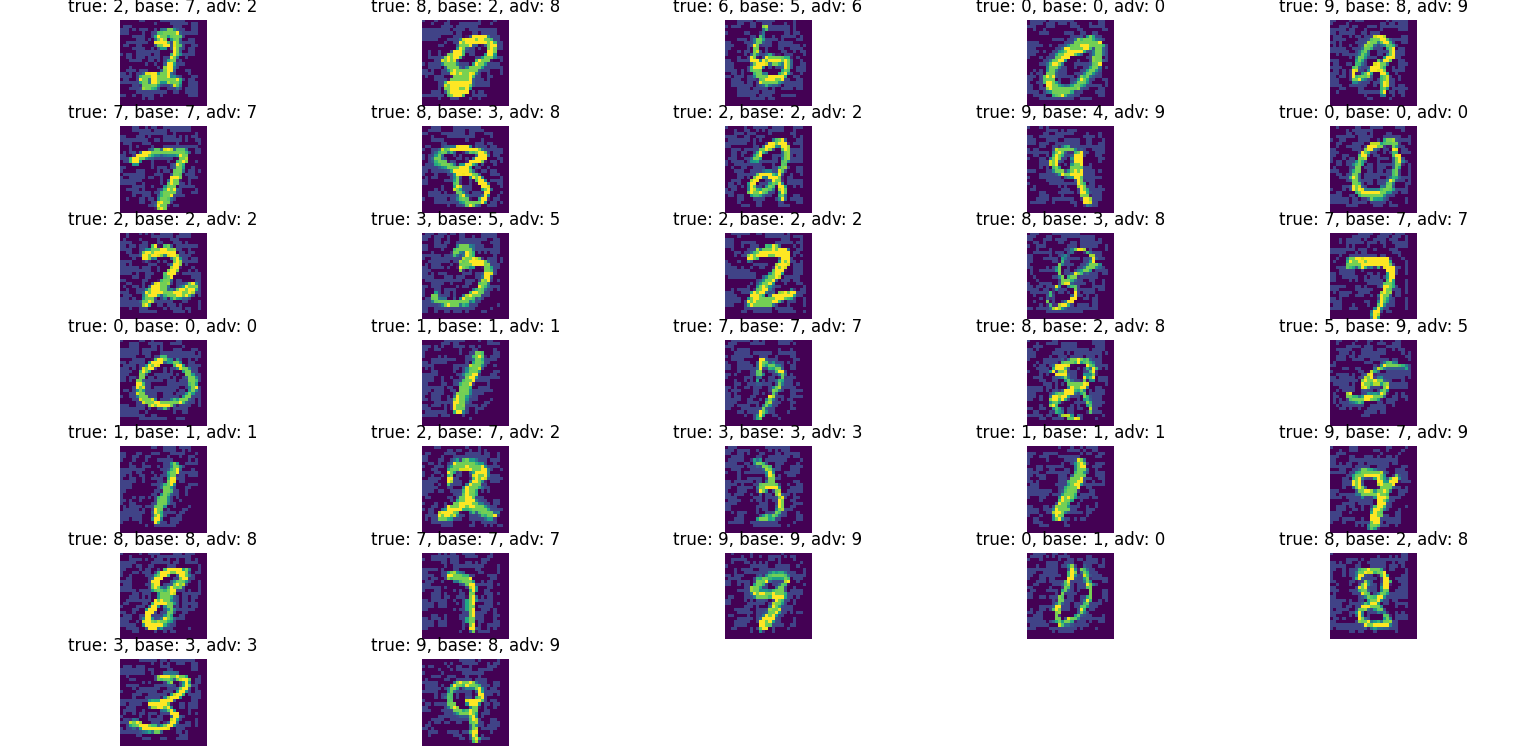
\includegraphics[width=\textwidth]{Image/result.png}
    \caption{Một số mẫu nhiễu loạn đối nghịch và các phán đoán của hai mô hình.}
    \label{fig 2.6:Một số mẫu nhiễu loạn đối nghịch và các phán đoán của hai mô hình.}
    
\end{figure}

\begin{figure}[h!]
    \centering
    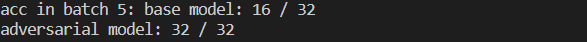
\includegraphics[width=\textwidth]{Image/acc_in_batch.png}
    \caption{Số dự đoán chính xác của hai mô hình trên mẫu nhiễu loạn đối nghịch trong batch 5.}
    \label{fig 2.7:Số dự đoán chính xác của hai mô hình trên mẫu nhiễu loạn đối nghịch trong batch 5.}
    
\end{figure}

Từ hình 2.6 ta thấy, các nhiễu loạn nhỏ được thêm vào những bức ảnh chữ số viết tay dưới mắt người vẫn có thể nhận biết được
tuy nhiên nó đã đánh lừa được mô hình cơ bản phán đoán sai.

Từ hình 2.7 ta thấy rằng, khả năng phán đoán của mô hình cơ bản(base model) khá thấp(21/32 mẫu). Trong khi đó
mô hình Adversarial-regularized phán đoán rất tốt (32/32 mẫu).


\textbf{Lưu mô hình vừa đào tạo}

Sau khi đào tạo chúng ta sẽ lưu lại các mô hình để thử cho các mô hình phán đoán một số hình ảnh viết tay không phải thuộc tập dữ
liệu của tensorflow\_datasets. Mô hình được lưu lại có thể dễ dàng mang ra sử dụng hoặc tiếp tục đào tạo tùy mục đích và no được lưu dưới định dạng '.h5' với sự hỗ trợ của
thư viện \textbf{h5py}. Lưu ý rằng, sau khi lưu mô hình thì các biến mà mô hình đã học tập được sẽ được giữ nguyên.

\begin{lstlisting}[language = Python]
    model_adv.save('Model/advs_model.h5')
    model_base.save('Model/base_model.h5')
\end{lstlisting}

\cite*{WEBSITE}

\subsection{Kiểm tra mô hình với một số ảnh viết tay}

Ở phần trước, chúng ta đã xây dựng, đào tạo và kiểm tra mô hình trên tập dữ liệu của tensorflow\_datasets. Tuy nhiên, chúng ta 
để biết được thực sự mô hình có hoạt động tốt với các bức ảnh ngẫu nhiên hay không, ta sẽ viết tay một số chữ số và cho mô hình dự đoán.

Ở phần này, chúng ta sẽ sử dụng thư viện xử lý ảnh OpenCV để đọc và tiền xử lý các bức ảnh chụp. Do đầu vào của mô hình là một bức ảnh 28x28
nên chúng ta cần phải resize ảnh về kích thước này. Sau đó, chúng ta cũng cần chuyển ảnh về dạng mảng numpy với giá trị trong khoảng 0-1 để mô hình ổn định hơn và 
tiến hành cho mô hình dự đoán.

\textbf{Import thư viện}

Các thư viện này đã được yêu cầu cài đặt trong file Setup.txt nên chỉ cần import vào là có thể sử dụng.
\begin{lstlisting}[language = Python]
    import cv2
    import numpy as np
    import tensorflow as tf
\end{lstlisting}

\textbf{Đọc ảnh và tiền xử lý ảnh}

Các bức ảnh chụp chữ số viết tay sẽ được lưu lại trong thư mục Image/. Chúng ta sẽ đọc các bức ảnh này và tiền xử lý để cho mô hình dự đoán.

\begin{lstlisting}[language = Python]
    image = cv2.imread("Image/test2.jpg")
    copy = image.copy()

    im_gray = cv2.cvtColor(image,cv2.COLOR_BGR2GRAY)
    im_blur = cv2.GaussianBlur(im_gray,(5,5),0)
    im,thre = cv2.threshold(im_blur,90,255,cv2.THRESH_BINARY_INV)
    contours,hierachy = cv2.findContours(thre,cv2.RETR_EXTERNAL,cv2.CHAIN_APPROX_SIMPLE)
    rects = [cv2.boundingRect(cnt) for cnt in contours]

\end{lstlisting}

Chúng ta sẽ đọc các bức ảnh này bằng hàm \textbf{imread()} có sẵn trong opencv sau đó sẽ copy ảnh vừa đọc và gán vào biến copy để sử dụng cho sau này.
Tiếp theo ta cần chuyển ảnh về dưới dạng thang xám để dễ dàng xử lý hơn bằng hàm \textbf{cvtColor()}.
Sau đó, chúng ta sẽ làm mờ ảnh bằng hàm \textbf{GaussianBlur()} để loại bỏ các nhiễu trong ảnh và tăng khả năng phán đoán chính xác của các mô hình.
Cuối cùng ta sẽ chuyển ảnh về dưới dạng nhị phân để có thể đưa vào mô hình dự đoán.

Do ảnh chụp có thể có nhiều chữ số viết tay nên chúng ta cần phải tách các chữ số ra. Để làm được điều này, chúng ta sẽ sử dụng hàm \textbf{findContours()} 
để tìm vị trí chuỗi số và các đường viền của các chữ số trong ảnh. Sau đó, chúng ta sẽ sử dụng hàm \textbf{boundingRect()} để tao các hình chữ nhật bao quanh các chữ số trong ảnh.

\textbf{Gọi mô hình và dự đoán}

Sau khi đã chuẩn bị các dữ liệu ảnh cần thiết, chúng ta sẽ gọi mô hình đã được train trước đó và dự đoán kết quả.

\begin{lstlisting}[language = Python]
    adv_model = tf.keras.models.load_model("Model/advs_model.h5")
    base_model = tf.keras.models.load_model("Model/base_model.h5")

    for i in contours:
        (x,y,w,h) = cv2.boundingRect(i)
        cv2.rectangle(image,(x,y),(x+w,y+h),(0,255,0),3)
        subImage = thre[y:y+h,x:x+w]
        subImage = np.pad(subImage,(20,20),'constant',constant_values=(0,0))
        subImage = cv2.resize(subImage, (28, 28), interpolation=cv2.INTER_AREA)
        subImage = cv2.dilate(subImage, (3, 3))

        img = subImage.reshape(1,28,28,1)
        img = img/255.0
        img = img.astype(np.float32)
        
        adv_pred = adv_model.predict(img)
        adv_pred = np.argmax(adv_pred)
        cv2.putText(copy,str(int(adv_pred)),(x,y+160),0,1,(0,0,255),2)

        base_pred = base_model.predict(img)
        base_pred = np.argmax(base_pred)
        cv2.putText(copy,str(int(base_pred)),(x,y+200),0,1,(0,255,0),2)

    cv2.imshow("image",copy)
    cv2.waitKey(0)


\end{lstlisting}

Sử dụng hàm \textbf{load\_model()} để gọi mô hình đã được train trước đó. Sau đó, chúng ta sẽ sử dụng vòng lặp để duyệt qua các chữ số trong ảnh.
Lúc này chúng ta vẫn chỉ có các ảnh thô dạng nhị phân của từng chữ số nên ta cần xử lý chúng, sử dụng hàm \textbf{resize} để chuyển ảnh về kích thước 28x28.
Tuy nhiên, đầu vào của các mô hình là ảnh có kích thước 28x28x1 nên ta cần chuyển ảnh về dạng một chiều. Để làm được điều này, chúng ta sẽ sử dụng hàm \textbf{reshape()}.
Sau đó, chúng ta sẽ chuẩn hóa ảnh về dạng 0-1 bằng cách chia cho 255.0. Cuối cùng, chúng ta sẽ sử dụng hàm \textbf{predict()} để dự đoán chữ số, và dự đoán đó sẽ được hiển 
thị lên bức ảnh copy từ trước. Dự đoán của mô hình cơ bản sẽ có màu xanh lá cây, còn dự đoán của mô hình Adversarial-regularized sẽ có màu đỏ.

\textbf{Kết quả dự đoán}

\begin{figure}[h]
    \centering
    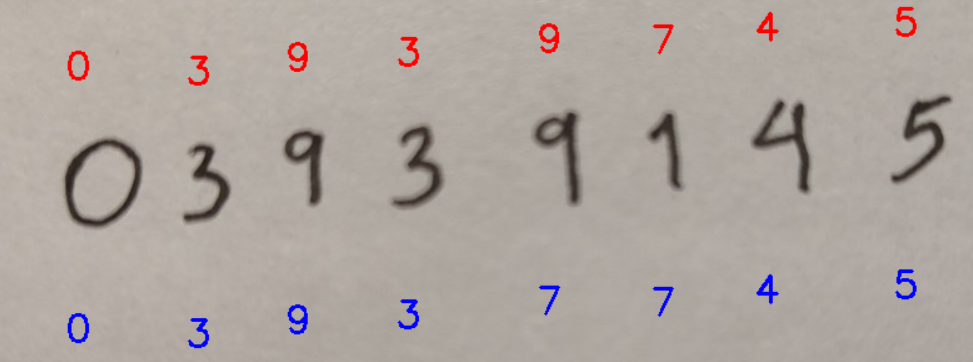
\includegraphics[width=\textwidth]{Image/test1.png}

    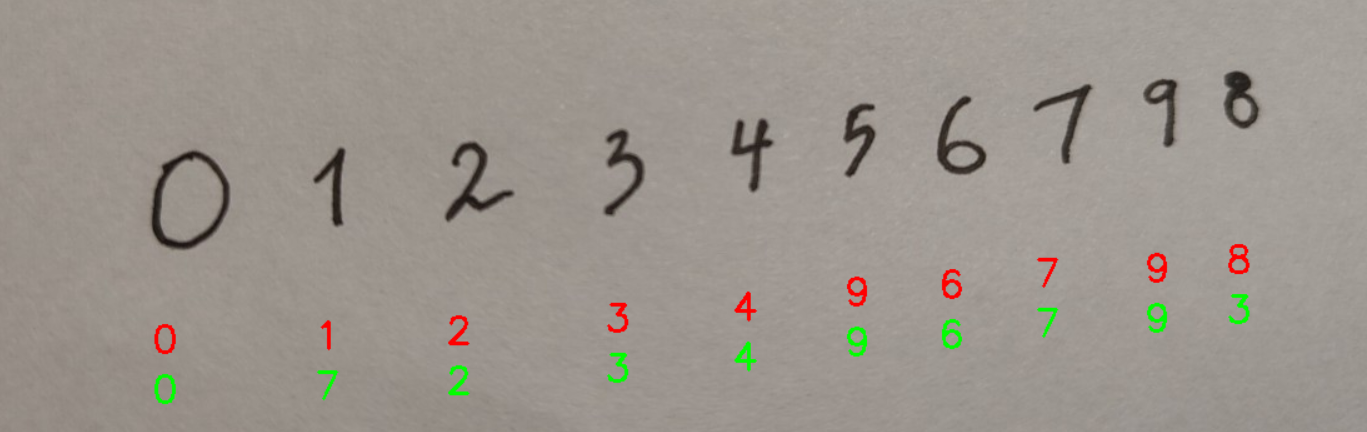
\includegraphics[width=\textwidth]{Image/test2.png}
    \caption{Kết quả dự đoán}
    \label{fig 2.8:Kết quả dự đoán}
\end{figure}

Từ hình 2.8 ta thấy. Ở bức ảnh phía trên, khi các chữ số được viết khá rõ ràng thì cả hai mô hình đều đưa ra dự đoán sai 1 chữ số.
Tuy nhiên ở hình dưới, khi các chữ số bị viết xấu hơn, các nét viết nguệch ngoạc thì mô hình Adversarial-regularized chỉ dự đoán sai 1/10 chữ số, trong khi mô hình cơ bản dự đoán sai 3/10 chữ số.
Từ đó ta thấy rằng, mô hình Adversarial-regularized có độ chính xác cao hơn và hoạt động tốt hơn mô hình cơ bản khi dữ liệu bị nhiễu. Và đây là một trong những ưu điểm của mô hình Adversarial-regularized.

